\documentclass{article}
\usepackage[utf8]{inputenc}
\usepackage{geometry}
\usepackage[usenames,dvipsnames,svgnames,table]{xcolor}
%\usepackage{color}
\usepackage{graphicx}
\usepackage{amsmath}
\usepackage{amsfonts}
\usepackage{url}
\usepackage{mathabx}
\usepackage{braket}
\usepackage{commath}
\usepackage{bbold}

\geometry{textwidth=6.5in, textheight=9.0in,
    marginparsep=7pt, marginparwidth=.6in}
\setlength{\parindent}{0in}
\setlength{\parskip}{0.08in}

\newcommand{\red}[1]{\textcolor{red}{#1}}
\newcommand{\blue}[1]{\textcolor{blue}{#1}}
\newcommand*{\annot}[1]{\tag*{\footnotesize{\textcolor{gray}{#1}}}}
\newcommand{\like}{\mathcal{L}}
\let\Pr\undefined
\DeclareMathOperator{\R}{R}

\title{Fourier planes}
\author{Josh Meyers}
\date{April 2018}

\begin{document}

\section{Intro}

The goal of this note is to A) write down how I think the HuygensPSF tool in Zemax works, (which is
also the description of how it works in my raytracing software \textsc{batoid}), and B) connect that
HuygensPSF description to Fourier optics, especially the relationships between the various 2D grids
of points (lattices) that arise in Fourier optics.

\section{HuygensPSF}

The Huygens construction electric field amplitude given a set of monochromatic plane waves $K$
evaluated at a particular time $t$ and location $\vec{x}$ is:

\begin{equation}
    A(\vec{x}, t) \propto \sum_{\vec{k} \in K} \exp\left(i \phi_{\vec{k}}\right) \exp\left( i \vec{k} \cdot \vec{x} - \omega t\right)
    \label{eqn:Huygens}
\end{equation}

In the above, I use $\vec{k}$ both as an index over different plane waves and to indicate the
wave vector of an individual plane wave.  The phase of each plane wave is given by $\phi_{\vec{k}}$,
and the temporal frequency of each wave is $\omega$.

Note that the input to the sum and therefore the resultant amplitude are both scalars.  I.e., I'm
asserting a scalar diffraction theory.  A more accurate vector diffraction theory would replace the
$\exp\left(\phi_{\vec{k}}\right)$ with something like $\vec{E}_{\vec{k}} \exp\left(i
\phi_{\vec{k}}\right)$ and the resulting amplitude would also be a vector quantity.

The PSF intensity given by \ref{eqn:Huygens} is then given by the square of the electric field
amplitude, which in our scalar field theory is:

\begin{equation}
    I(\vec{x}) = I(\vec{x}, t) = |A(\vec{x}, t)|^2
\end{equation}

Note that the time dependence drops out in the amplitude-squared operation.  Given the above, the
whole trick then is to figure out what is the set $K$.

\section{Lattices}

I will use the word "lattice" to refer to a two dimensional set of points that are uniformly
distributed in the plane on a grid, which may be square or rectilinear, but is not required to be.
(I.e., a Bravais lattice as borrowed from solid-state physics.) Concretely, the lattice $L$ is the
set of points:

\begin{equation}
    L = \Set{\vec{\ell}_1 \mathrm{i} + \vec{\ell}_2 \mathrm{j} | \mathrm{i},\mathrm{j} \in \mathbb{Z} \times \mathbb{Z}}
\end{equation}

where $\vec{\ell}_1$ and $\vec{\ell}_2$ are the "primitive lattice vectors", whose only constraint,
I believe, is that they are linearly independent.  In particular, they need not be unit vectors or
orthogonal to each other.  (Note also the use of romanized $\mathrm{i}$ and $\mathrm{j}$ as indices,
distinct from the italicized $i$ used for the imaginary unit.)

In what follows, we will be interested in at least 5 different lattices, itemized below together
with their respective dimensions:

\begin{itemize}
    \item The pupil lattice $U$ [ length ]
    \item The focal plane lattice $X$ [ length ]
    \item The Fourier conjugate of the focal plane lattice $K_\mathrm{dft}$ [ inverse length ]
    \item The sky tangent plane lattice $\Theta$ [ angle ]
    \item The Fourier conjugate of the sky tangent plane $Q$ [ inverse angle ].
\end{itemize}

While the specific point grids of interest on the focal plane or on the sky won't generally include
the origin, for this note we'll ignore such origin shifts.   In fact, for Fourier optics we are
generally interested in just the lattice subsets for which $\mathrm{i},\mathrm{j} \in \mathbb{I}_N
\equiv [-N/2, ..., N/2-1] \times [-N/2, ..., N/2-1]$ for some natural number $N$.

\section{Pupil lattice}

We are interested in the PSF of an incoming plane wave.  We assume the intensity of the wave is
uniform over the telescope entrance pupil, which leads us to use a particularly simple lattice to
describe the entrance pupil plane, with primitive lattice vectors

\begin{equation}
    \vec{u}_1 = \Delta u \hat{\imath}
\end{equation}
and
\begin{equation}
    \vec{u}_2 = \Delta u \hat{\jmath}
\end{equation}

for some asserted sampling length $\Delta u$. (Note we are overloading the i and j characters again,
this time with hats to indicate they are unit vectors.)

We wouldn't necessarily need a square lattice for the pupil -- parallelograms would be okay, or even
a hexagonal "lattice" (uniformity is important though) --  but a square lattice is easy so we stick
with that for now.

We interpret each point in the pupil lattice as an incoming ray.  Because they represent a plane
wave, the rays' directions of propagation are all identical, forming some angle with the optic axis.
Furthermore, the rays' phases are identical along any plane perpendicular to their direction of
propagation.  The rays will propagate through the optical system of interest, each experiencing
different degrees of phase delays and changes in propagation direction.  If we can calculate or
model these changes, then we can reinterpret the rays as plane waves near the focal plane and use
Eq. \ref{eqn:Huygens} to determine the PSF at any location of interest.

\section{Paraxial Optics}

We'll first describe obtaining $K$ using paraxial optics, which basically means we assume that the
rays are close to the optic axis and $\sin \theta \approx \theta$.

\subsection{Focal Plane}

For the Huygens construction, we are free to choose the points $\vec{x} \in X$ at which to evaluate
the PSF, and, given a set of rays (= plane waves) can directly evaluate the sum Eq.
\ref{eqn:Huygens} at these locations.  Evaluating the sum directly can be slow, since it's linear in
both the number of rays used and the number of evaluation points.  In practice, we are usually
interested in a square lattice of rays (with say N rays on a side) and square lattice of evaluation
points (with M points on a side), so the direct sum is $O(M^2 N^2)$.  Fortunately, Eq.
\ref{eqn:Huygens} can, with a few approximations, be manipulated into the form of a 2D Discrete
Fourier transform, which can be evaluated in $O(N^2 \log N)$ time, provided we are able to give up
the freedom to choose both M and N independently.

The approximation enabling the use of a Fourier transform concerns the relation between a ray's
initial pupil coordinate $\vec{u}$ and its final wave vector component $\vec{k}$.  Figure
\ref{fig:wavevector} illustrates this relationship under paraxial optics.

\begin{figure}
    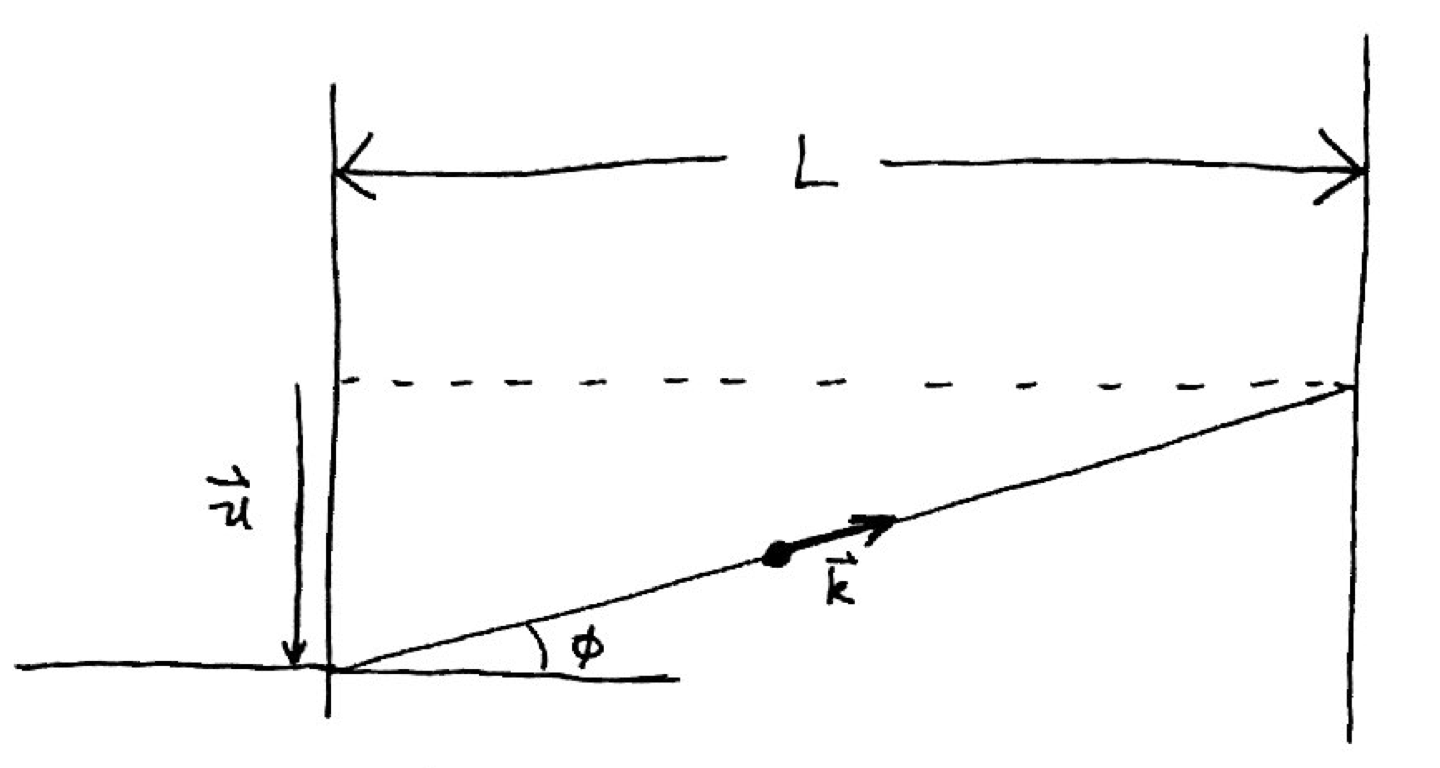
\includegraphics{wavevector.png}

    \caption{Relation between entrance pupil coordinate $\vec{u}$ and focal-plane-space wave vector
    $\vec{k}$ for a telescope with focal length $L$.  A plane wave enters from the left where it
    encounters the entrance pupil, and gets focused to the right at the focal plane.}

    \label{fig:wavevector}
\end{figure}

For pupil coordinates close to the optic axis (the paraxial approximation), we have

\begin{equation}
    \frac{\vec{k}}{|\vec{k}|} = -\frac{\vec{u}}{\sqrt{|\vec{u}|^2 + L^2}} \approx -\frac{\vec{u}}{L}
\end{equation}

or

\begin{equation}
    \vec{k} \approx -\frac{2 \pi}{\lambda n}\frac{\vec{u}}{L}
    \label{eqn:kuapprox}
\end{equation}

If we use this relation, we can construct a uniform rectilinear grid of $\vec{k}$ vectors
(specifically, the x and y components of $\vec{k}$) that directly correspond the the initial
rectilinear $\vec{u}$ vectors.  I.e., the primitive lattice vectors for $\vec{k}$ are:

\begin{equation}
    \vec{k}_1 = -\frac{2 \pi}{\lambda n L} \vec{u}_1
\end{equation}
and
\begin{equation}
    \vec{k}_2 = -\frac{2 \pi}{\lambda n L} \vec{u}_2
\end{equation}

With this lattice, we can rewrite Eq. \ref{eqn:Huygens} as

\begin{equation}
    A(\vec{x}) \propto \sum_{\mathrm{i},\mathrm{j} \in \mathbb{I}} P_{\mathrm{ij}}
        \exp\left(i \phi_{\mathrm{ij}}\right)
        \exp\left(i \vec{k}_{\mathrm{ij}}\cdot \vec{x}\right).
\end{equation}

where $P_{\mathrm{ij}}$ indicates vignetted (0) or unvignetted (1) rays.

With the proper choice for a grid of $\vec{x}$ coordinates, we recognize the above as a 2D discrete
Fourier transform.

For GalSim, the convention for the discrete Fourier transform between lattices with primitive vectors
$\{\vec{a}_1, \vec{a}_2\}$ and $\{\vec{b}_1, \vec{b}_2\}$ (and N points each) are that

\begin{equation}
    b_i a_i = \frac{2 \pi}{N}, i \in \{1, 2\}
    \label{eqn:rectReciprocal}
\end{equation}

A slightly more general relation that allows for lattices with uniform but non-rectilinear grids is
obtained from the reciprocal lattice formalism in solid-state physics.  (E.g., see
\url{https://physics.stackexchange.com/questions/340860/reciprocal-lattice-in-2d}) For GalSim DFTs,
this becomes:

\begin{equation}
    \vec{b}_i \cdot \vec{a}_j = \frac{2 \pi}{N} \delta_{ij}
    \label{eqn:reciprocal}
\end{equation}

For paraxial optics though, we simply take focal plane space primitive lattice vectors resulting
from Eq. \ref{eqn:rectReciprocal}:

\begin{equation}
    \vec{x}_1 = -\frac{\lambda n L}{N \Delta u} \hat{\imath}
\end{equation}

\begin{equation}
    \vec{x}_2 = -\frac{\lambda n L}{N \Delta u} \hat{\jmath}
\end{equation}

which allow us to write

\begin{equation}
    A(\vec{x}_{\mathrm{pq}}) \propto \sum_{\mathrm{i},\mathrm{j} \in \mathbb{I}}
        P_{\mathrm{ij}}
        \exp\left(i \phi_{\mathrm{ij}}\right)
        \exp\left(i \vec{k}_{\mathrm{ij}}\cdot \vec{x}_{\mathrm{pq}}\right).
\end{equation}

or

\begin{equation}
    A(\vec{x}_{\mathrm{pq}}) \propto
        \left[\mathrm{DFT}\left(P_{\mathrm{ij}} \exp\left(i \phi_{\mathrm{ij}} \right) \right)\right]_{\mathrm{pq}}
\end{equation}

\subsection{Sky plane}

The previous subsection tells us how to compute the PSF intensity under Fourier optics on the focal
plane, where the dimensions on the focal plane are in length.  We are also interested, however, in
the PSF intensity distribution as projected on the sky.  For this, we need the plate scale of the
telescope.

\begin{figure}
    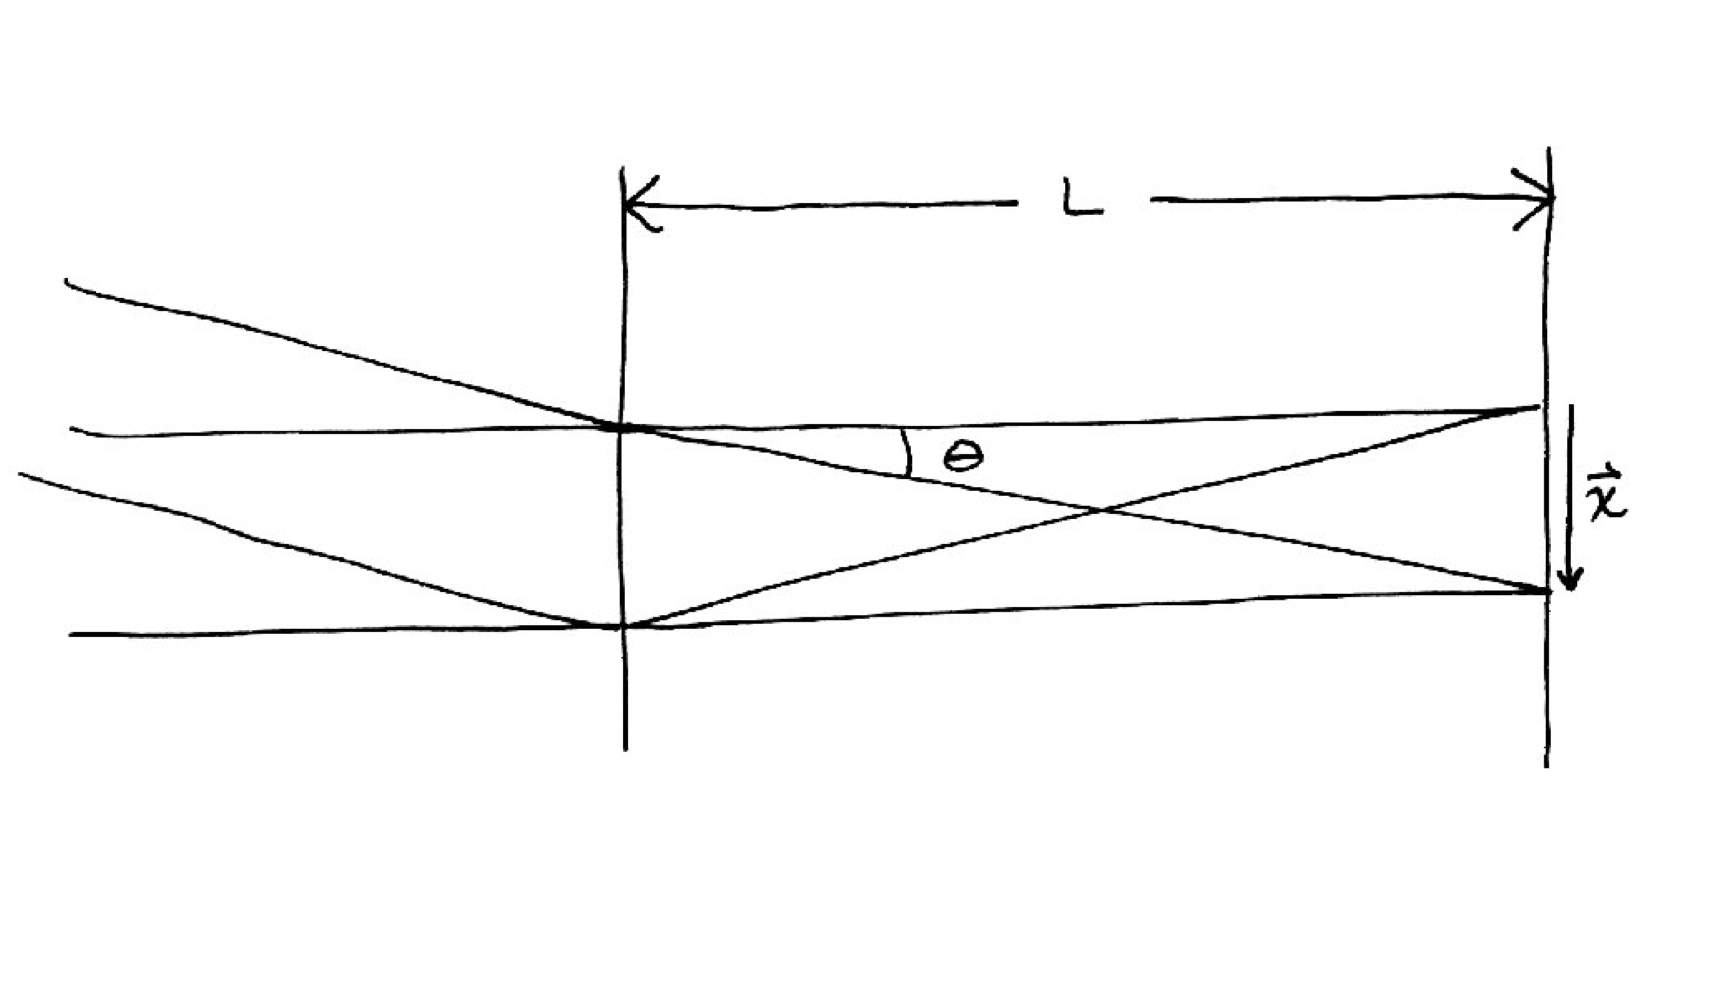
\includegraphics{PlateScale.png}
    \caption{Toy telescope model for determining the plate scale.}
    \label{fig:PlateScale}
\end{figure}

Again, using a toy model, we can get an approximate relation between focal plane coordinates and sky
coordinates.  Figure \ref{fig:PlateScale} shows that this relation is

\begin{equation}
    \vec{\theta} = \hat{\theta} \arctan \frac{|\vec{x}|}{L} \approx \frac{\vec{x}}{L}
\end{equation}

where $\vec{\theta}$ is the angle on the sky (say, a 2d tangent plane projection),  the telescope
focal length is again $L$, and the focal plane coordinate is $\vec{x}$.  We can thus use sky-plane
primitive lattice vectors:

\begin{equation}
    \vec{\theta_1} = -\frac{\lambda n}{N \Delta u} \hat{\imath}
\end{equation}

\begin{equation}
    \vec{\theta_2} = -\frac{\lambda n}{N \Delta u} \hat{\jmath}
\end{equation}

The telescope focal length conveniently divides out.

Ignoring the refractive index $n$, this is equivalent to the GalSim convention of

\begin{equation}
    \Delta \theta = \frac{\lambda}{N \Delta u}
\end{equation}

We'll label the Fourier conjugate of the sky-coordinate $\vec{\theta}$ as $\vec{q}$.  Using the same
reciprocal lattice formalism as before, we find that the sky-plane Fourier lattice has primitive
vectors

\begin{equation}
    \vec{q_1} = -\frac{2 \pi \Delta u}{\lambda n} \hat{\imath}
\end{equation}
\begin{equation}
    \vec{q_2} = -\frac{2 \pi \Delta u}{\lambda n} \hat{\jmath}
\end{equation}

Ignoring the refractive index, this is equivalent (up to a minus sign) to the GalSim convention of

\begin{equation}
    \Delta q = \frac{2 \pi}{\lambda} \Delta u
\end{equation}

\section{Non-paraxial optics}

Paraxial optics are great fun, but don't tell the entire story, especially for a telescope with a
wide field of view and a fast beam.  Here, we look at more precise relationships between the various
planes of interest, determined by tracing rays.

\subsection{Focal plane}

Leaving the grid on the pupil plane the same as in the paraxial case, our first difference for more
precise optics concerns the relation between the pupil plane and the Fourier conjugate to the image
plane; i.e., $\vec{k}(\vec{u})$.  Figure \ref{fig:ku} shows the relationship between $\vec{k}$ and
$\vec{u}$ for the Subaru/HSC telescope and camera for an incoming plane wave tilted 0.01 radians to
the optic axis in the +y direction, determined using the raytracing software \textsc{batoid}.  The
relationship is quite linear as expected.

\begin{figure}
    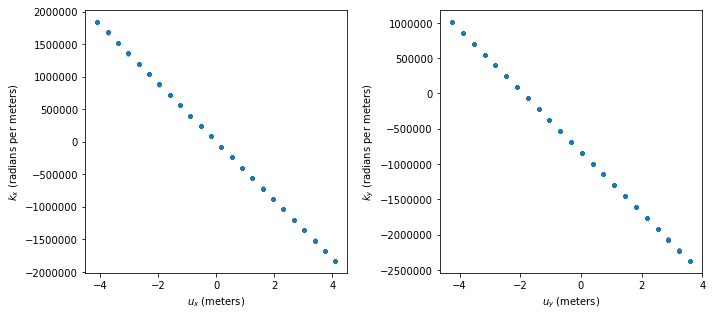
\includegraphics[scale=0.7]{ku.png}

    \caption{Relation between entrance pupil coordinate in meters and wave vector component at the
    focal plane in radians of phase per meter. The relationship is nearly linear.  Note that the
    relationship does not pass through the origin in the y-direction, which is related to the degree
    of non-telecentricity of the Subaru/HSC system when the incoming plane wave is tilted in y.}

    \label{fig:ku}
\end{figure}

To determine just how linear the relations are, we show the residuals to bilinear fits of $k_x$ and
$k_y$ against $u_x$ and $u_y$ in figure \ref{fig:dku}.  The coefficients in the fit (ignoring the
constant piece), are the Jacobian of the transformation between $\vec{u}$ and $\vec{k}$.  For this
particular situation, this Jacobian is:


\begin{gather}
 \frac{\partial \vec{k}}{\partial \vec{u}}
 =
  \begin{bmatrix} \frac{\partial k_x}{\partial u_x} & \frac{\partial k_x}{\partial u_y} \\
                  \frac{\partial k_y}{\partial u_x} & \frac{\partial k_y}{\partial u_y} \end{bmatrix}
 =
  \begin{bmatrix}
   -4.5 \cdot 10^5 & 6.2 \cdot 10^{-2} \\
   2.1 \cdot 10^{-1} & -4.3 \cdot 10^5
   \end{bmatrix}
\end{gather}

(in units of radians of phase per meter squared).

\begin{figure}
    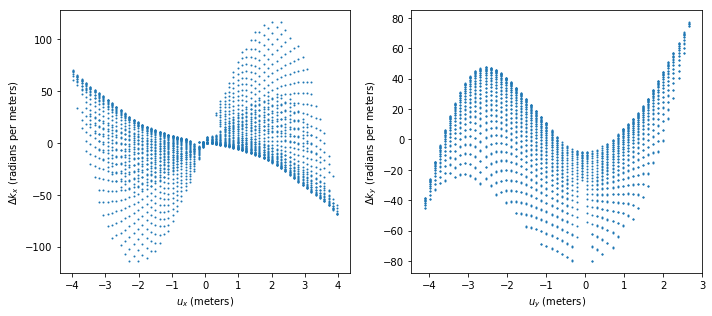
\includegraphics[scale=0.7]{dku.png}

    \caption{Relation between entrance pupil coordinate and the residual to a linear fit of the
    wavevector component against both pupil coordinate components.  Note the y-axis scale is a
    factor of $\sim 10^4$ smaller than in the previous figure.}

    \label{fig:dku}
\end{figure}

The diagonal components are close to the predicted value from the paraxial approximation of

\begin{equation}
    -\frac{2 \pi}{\lambda n L} = -5.6 \cdot 10^5 \mathrm{\,rad\,m^{-2}}
\end{equation}

where I used 15 $m$ as the focal length (possibly too short).  However, it's notable that the
diagonal components are not the \textit{same}.  In particular, using $\vec{k} = \frac{\partial
\vec{k}}{\partial \vec{u}} \vec{u}$ and Eq. \ref{eqn:reciprocal}, we find

\begin{equation}
    \vec{x}_1 =
\end{equation}

\begin{equation}
    \vec{x}_2 =
\end{equation}

\subsection{Sky plane}



\section{TODO}

\begin{itemize}
    \item Explicitly write out $\tilde{I}\left(\vec{q}\right)$
    \item Add plots and commentary of $\vec{\theta}$ vs $\vec{x}$.
\end{itemize}

\end{document}
